% ../../../1994_全国卷_文科/figures/f1994_national_arts_q12_inverse_graphs.tex — 1994 年·全国卷·文科 第 12 题（四图象选项）
%
% 【来源】`.work/phase4-b19/source/1994全国文.pdf`（SHA-256 68085b2f5b0285e127f63c87f6737434fddb156cbc4689b8957c2a4be4bb1bda），第 1 页；
%   内容流逐路径照录，本地坐标 = 页面坐标 − (458.700,608.330)，1 单位 = 1 TeX pt。
%   每个 m 子路径独立起笔；线宽/虚线按内容流原值；标签取 pdftotext -bbox 中心。
%
% 元素计数：24 路径＋24 标签
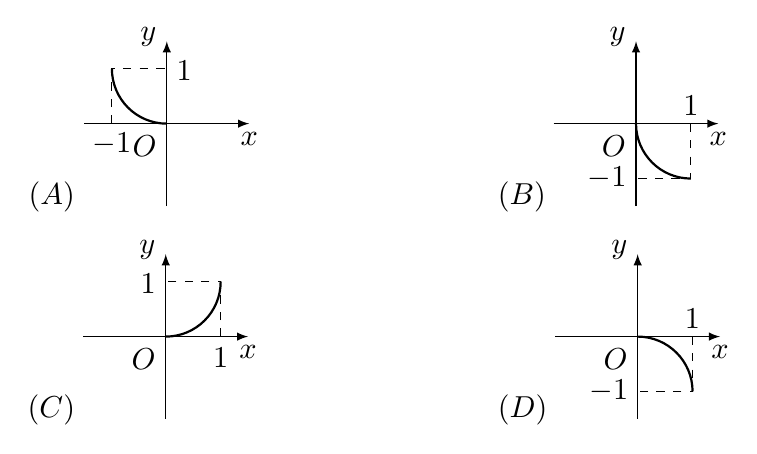
\begin{tikzpicture}[x=1pt, y=1pt,
    every node/.style={inner sep=0pt, font=\fontsize{10.5pt}{12.6pt}\selectfont}]
  \draw[line width=0.398pt] (0.378,106.710) -- (56.319,106.710);
  \fill[line width=1.0pt] (59.906,106.710) .. controls (58.843,106.909) and (57.116,107.507) .. (55.921,108.204) -- (55.921,105.216) .. controls (57.116,105.913) and (58.843,106.511) .. (59.906,106.710);
  \draw[line width=0.398pt] (30.142,76.946) -- (30.142,132.887);
  \fill[line width=1.0pt] (30.142,136.474) .. controls (29.943,135.411) and (29.345,133.684) .. (28.648,132.489) -- (31.636,132.489) .. controls (30.939,133.684) and (30.341,135.411) .. (30.142,136.474);
  \draw[line width=0.398pt, dash pattern=on 2.989pt off 2.989pt] (10.299,106.710) -- (10.299,126.553) -- (30.142,126.553);
  \draw[line width=0.797pt] (30.142,106.710) .. controls (19.183,106.710) and (10.299,115.594) .. (10.299,126.553);
  \draw[line width=0.398pt] (169.928,106.710) -- (225.869,106.710);
  \fill[line width=1.0pt] (229.456,106.710) .. controls (228.393,106.909) and (226.666,107.507) .. (225.471,108.204) -- (225.471,105.216) .. controls (226.666,105.913) and (228.393,106.511) .. (229.456,106.710);
  \draw[line width=0.398pt] (199.692,76.946) -- (199.692,132.887);
  \fill[line width=1.0pt] (199.692,136.474) .. controls (199.493,135.411) and (198.895,133.684) .. (198.198,132.489) -- (201.186,132.489) .. controls (200.489,133.684) and (199.891,135.411) .. (199.692,136.474);
  \draw[line width=0.398pt, dash pattern=on 2.989pt off 2.989pt] (219.535,106.710) -- (219.535,86.867) -- (199.692,86.867);
  \draw[line width=0.797pt] (199.692,106.710) .. controls (199.692,95.751) and (208.576,86.867) .. (219.535,86.867);
  \draw[line width=0.398pt] (-0.004,29.761) -- (55.937,29.761);
  \fill[line width=1.0pt] (59.524,29.761) .. controls (58.461,29.960) and (56.734,30.558) .. (55.539,31.255) -- (55.539,28.267) .. controls (56.734,28.964) and (58.461,29.562) .. (59.524,29.761);
  \draw[line width=0.398pt] (29.760,-0.003) -- (29.760,55.938);
  \fill[line width=1.0pt] (29.760,59.525) .. controls (29.561,58.462) and (28.963,56.735) .. (28.266,55.540) -- (31.254,55.540) .. controls (30.557,56.735) and (29.959,58.462) .. (29.760,59.525);
  \draw[line width=0.398pt, dash pattern=on 2.989pt off 2.989pt] (49.603,29.761) -- (49.603,49.604) -- (29.760,49.604);
  \draw[line width=0.797pt] (29.760,29.761) .. controls (40.719,29.761) and (49.603,38.645) .. (49.603,49.604);
  \draw[line width=0.398pt] (170.516,29.761) -- (226.457,29.761);
  \fill[line width=1.0pt] (230.044,29.761) .. controls (228.981,29.960) and (227.254,30.558) .. (226.059,31.255) -- (226.059,28.267) .. controls (227.254,28.964) and (228.981,29.562) .. (230.044,29.761);
  \draw[line width=0.398pt] (200.280,-0.003) -- (200.280,55.938);
  \fill[line width=1.0pt] (200.280,59.525) .. controls (200.081,58.462) and (199.483,56.735) .. (198.786,55.540) -- (201.774,55.540) .. controls (201.077,56.735) and (200.479,58.462) .. (200.280,59.525);
  \draw[line width=0.398pt, dash pattern=on 2.989pt off 2.989pt] (220.123,29.761) -- (220.123,9.918) -- (200.280,9.918);
  \draw[line width=0.797pt] (200.280,29.761) .. controls (211.239,29.761) and (220.123,20.877) .. (220.123,9.918);
  \node[anchor=center] at (23.490,137.970) {$y$};
  \node[anchor=center] at (59.910,101.230) {$x$};
  \node[anchor=center] at (22.150,98.570) {$O$};
  \node[anchor=center] at (36.470,125.900) {$1$};
  \node[anchor=center] at (10.300,99.500) {$-1$};
  \node[anchor=center] at (-11.430,80.070) {$(A)$};
  \node[anchor=center] at (193.040,137.970) {$y$};
  \node[anchor=center] at (229.460,101.230) {$x$};
  \node[anchor=center] at (191.700,98.570) {$O$};
  \node[anchor=center] at (219.540,113.140) {$1$};
  \node[anchor=center] at (189.280,87.180) {$-1$};
  \node[anchor=center] at (158.430,80.070) {$(B)$};
  \node[anchor=center] at (23.110,61.020) {$y$};
  \node[anchor=center] at (59.520,24.280) {$x$};
  \node[anchor=center] at (21.760,21.620) {$O$};
  \node[anchor=center] at (23.440,48.950) {$1$};
  \node[anchor=center] at (49.600,22.030) {$1$};
  \node[anchor=center] at (-11.570,3.120) {$(C)$};
  \node[anchor=center] at (193.630,61.020) {$y$};
  \node[anchor=center] at (230.040,24.280) {$x$};
  \node[anchor=center] at (192.280,21.620) {$O$};
  \node[anchor=center] at (220.120,36.190) {$1$};
  \node[anchor=center] at (189.870,10.230) {$-1$};
  \node[anchor=center] at (158.730,3.120) {$(D)$};
\end{tikzpicture}
%
% 【自验结果】逐路径照录；探针编译 0 警告。
